% !TEX TS-program = XeLaTeX
% !TEX spellcheck = en-US
\documentclass[aspectratio=169]{beamer}

\usetheme{bi}

\title{Lecture 5:\\ Model selection, evaluation and assessment}
\institute{GRA4160: Predictive modelling with machine learning}
\date{February 8th 2023}
\author{Vegard H\o ghaug Larsen}

\begin{document}

\maketitle

\frame{
	\frametitle{Plan for today:}
    \begin{enumerate}
		\item Model selection, evaluation and assessment
		\item Information criteria
		\item Cross-validation
		\item Bias-variance trade-off
    \end{enumerate}
}

\frame{
	\frametitle{Model selection}
	\begin{itemize}
		\item Model selection is the process of choosing the best model from a set of candidate models
		\pause
		\item The simplest approach is to compare the performance of different models on a held-out test set, and choose the model with the best performance
		\pause
		\item This approach can lead to overfitting, where the model that performs the best on the validation set is not the best model for the problem in general
		\pause
		\item \textbf{Cross-validation} is a more robust approach where we select the model that performs best on the validation set in each fold of the data
		\pause
		\item Another alternative is to use \textbf{inforation criteria} where we e.g., csn calculate the AIC or BIC value for each candidate model, and choose the model with the lowest value
	\end{itemize}
}

\frame{
	\frametitle{Model Evaluation}
	\begin{itemize}
		\item Model evaluation is the process of evaluating the performance of a model on new unseen data
		\pause
		\item This is typically done by dividing the data into training and testing sets, or by using cross-validation techniques
		\pause
		\item The goal of model evaluation is to determine how well the model is likely to perform in practice
		\pause
		\item Common metrics used for model evaluation include accuracy, precision, recall, ROC curve, and AUC
		\pause
		\item Visualizations such as confusion matrices and decision boundaries can also be useful for evaluating the performance of a model
	\end{itemize}
}

\frame{
	\frametitle{Metrics used for model evaluation}
	\begin{itemize}
		\item \textbf{Accuracy} is the fraction of predictions that are correct
		\pause
		\item \textbf{Precision} is the fraction of positive predictions that are correct
		\pause
		\item \textbf{Recall} measures the ability of a model to correctly identify all positive instances in a dataset
		\pause
		\item \textbf{ROC} curve is a plot of the true positive rate against the false positive rate
		\pause
		\item \textbf{AUC} is the area under the ROC curve
	\end{itemize}
	More details: See exercise 5 in the exercise notebook
}

\frame{
	\frametitle{Model Assessment}
	\begin{itemize}
		\item Model assessment is a broader concept that cover the evaluation of multiple aspects of a trained model
		\pause
		\item In addition to evaluating the  model's performance on new data, model assessment also refers to assessing factors such as the model's \textbf{complexity}, \textbf{interpretability}, \textbf{computational efficiency}, and \textbf{scalability}
		\pause
		\item Can involve conducting sensitivity analyses or stress tests to determine how the model performs under different conditions or scenarios.
	\end{itemize}
}

\frame{
	\frametitle{k-fold cross-validation}
	\begin{itemize}
		\item The original dataset is randomly partitioned into $k$ equal sized subsets or folds
		\pause
		\item The first fold is used as the test set and the remaining $k-1$  folds are used as the training set
		\pause
		\item This process is repeated $k$ times, with each of the $k$ folds used exactly once as the validation data
		\pause
		\item Can provide a more reliable estimate of the model's performance, as it uses all the data for both training and testing
		\pause
		\item Useful when the amount of data available is limited
	\end{itemize}

	\pause

Common on values of k are 5 and 10, but the choice of k depends on the size of the dataset and the computational resources available.
Larger values of k lead to more reliable estimates of the model's performance, but also increase the computational cost
}

\frame{
	\frametitle{The Bias-Variance tradeoff}

	\begin{itemize}
		\item A fundamental concept that relates to the performance of a model on new data
		\pause
		\item Bias refers to the degree to which a model's predictions deviate from the true values of the target variable
		\item High bias can result in underfitting, where the model is too simple to capture the underlying patterns in the data
		\pause
		\item Variance refers to the degree to which a model's predictions vary with changes in the training data
		\item High variance can result in overfitting, where the model is too complex and fits the training data too closely, leading to poor generalization to new data
		\pause
		\item The goal is to find a balance between bias and variance that results in a model that generalizes well to new data
	\end{itemize}
}


\frame{
	\frametitle{High bias and high variance}
	\begin{itemize}
		\item High variance refers to a model that overfits the training data
		\item High variance can be addressed by simplifying the model or by adding regularization techniques
		\pause
		\item High bias refers to a model that underfits the training data
		\item High bias can be addressed by using a more complex model, increasing the number of features, or reducing regularization
	\end{itemize}
}

\frame{
	\frametitle{Example of high bias}
	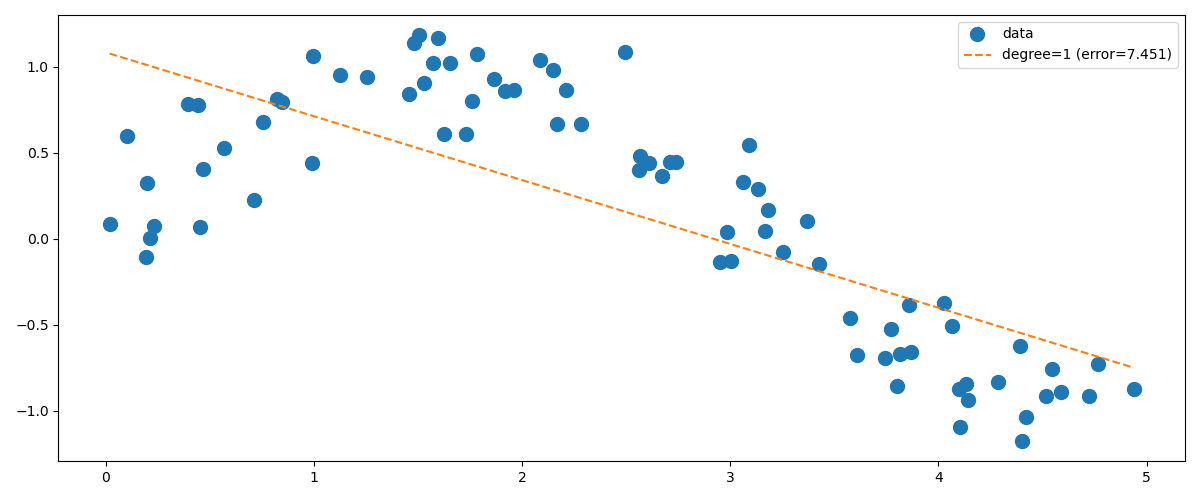
\includegraphics[scale=0.5]{figures/bias_variance_tradeoff_1.png}
}

\frame{
	\frametitle{Example of high variance}
    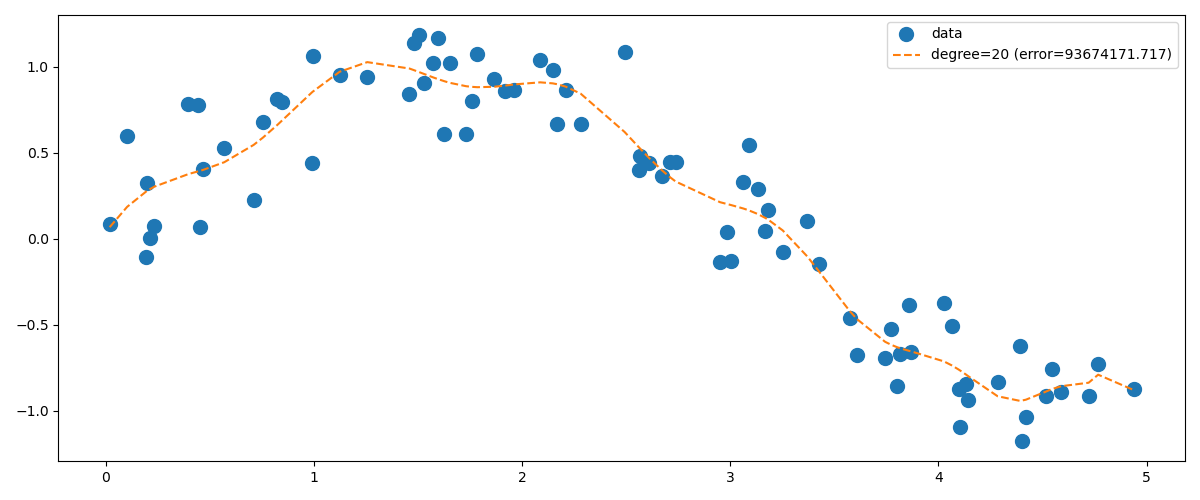
\includegraphics[scale=0.5]{figures/bias_variance_tradeoff_2.png}
}

\frame{
	\frametitle{Exercise: Model selection, assessment and evaluation}
\begin{itemize}
	\item Use cross-validation to evaluate the performance of a $k$-nearest neighbors (KNN) model trained on the iris dataset. Vary the number of neighbors and compare the resulting cross-validation scores. Which value of $k$ gives the best performance?
    \item Train different models on the iris dataset and compare their performance using accuracy and a confusion matrix. Which model performs best?
    \item Perform $k$-fold cross-validation on the iris data and compare the performance of several models such as KNN, decision trees, and logistic regression. Which model performs best?
    \item Train a decision tree on the iris dataset. Use \texttt{GridSearchCV} to find the best hyperparameters for \texttt{max\_depth}, \texttt{min\_samples\_leaf}, and \texttt{min\_samples\_split}. What is the model accuracy with optimized hyperparameters?
\end{itemize}
}

\end{document}